\begin{surferPage}{雙錐面}
    雙錐面(右圖)具有最簡單的奇異點。它是唯一一個能夠用二次多項式定義的奇異曲面:\[x^2+y^2-z^2=0.\]當把此等式右端的$0$用一個比較小的數$a\neq 0$替代後,雙錐面變化為雙曲面中的一種(由$a$的正負性決定):
    \begin{center}
      \begin{tabular}{@{}c@{\ }c@{\ }c@{\ }c@{\ }c@{}}
        \begin{tabular}{@{}c@{}}
          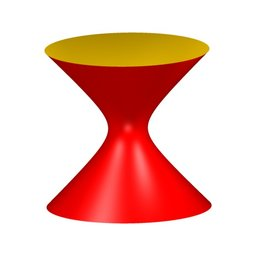
\includegraphics[width=1.2cm]{./../../common/images/A1pm_2}
        \end{tabular}
        &
        $\leftarrow$
        &
        \begin{tabular}{@{}c@{}}
          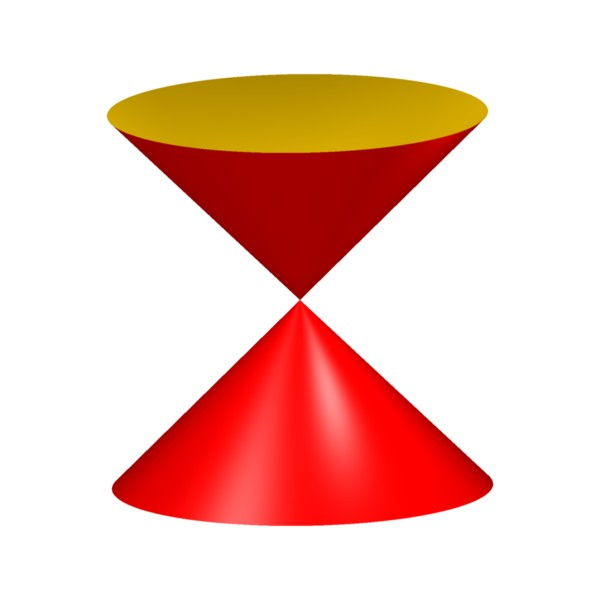
\includegraphics[width=1.2cm]{./../../common/images/A1pm_1}
        \end{tabular}
        &
        $\rightarrow$
        &
        \begin{tabular}{@{}c@{}}
          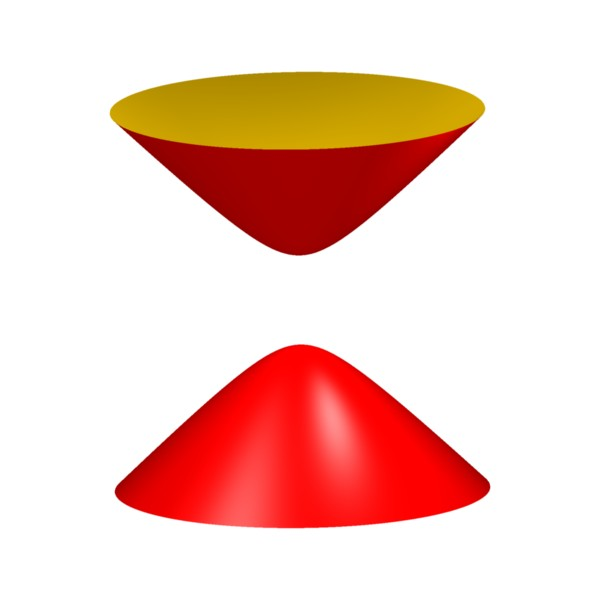
\includegraphics[width=1.2cm]{./../../common/images/A1pm_0}
        \end{tabular}
      \end{tabular}
    \end{center}
   一個二次曲面的奇異點數不可能多於$1$,即$\mu(2)=1$。
\end{surferPage}
